\documentclass[parskip,11pt,nochapterpage,bigchapter,linedtoc,colorback,accentcolor=tud1d,openany]{tudreport}
%\usepackage{ngerman}
\usepackage[english]{babel}

\usepackage[stable]{footmisc}
\usepackage[ngerman]{hyperref}

\usepackage{graphics}
\usepackage{caption}
\usepackage{subcaption}
\usepackage{longtable}
\usepackage{multirow}
\usepackage{booktabs}
\usepackage{listings}
\usepackage{hhline}
\usepackage{algorithm}
\usepackage{algpseudocode}
\usepackage{siunitx}

\usepackage{pgfplots}
\usepackage{pgfplotstable, booktabs}

\usepackage{xcolor}
\newcommand\myworries[1]{\textcolor{red}{#1}}

\graphicspath{{graphics/}}

\definecolor{codegray}{gray}{0.90}
\definecolor{pblue}{rgb}{0.13,0.13,1}
\definecolor{pgreen}{rgb}{0,0.5,0}
\definecolor{pred}{rgb}{0.9,0,0}
\definecolor{pgrey}{rgb}{0.46,0.45,0.48}

\lstdefinestyle{rawtext}{
  belowcaptionskip=4pt,
  captionpos=b
  breaklines=true,
  frame=N,
  xleftmargin=\parindent,
  language={},
  showstringspaces=false,
  basicstyle=\ttfamily,
  keywordstyle=\color{black},
  commentstyle=\color{black},
  identifierstyle=\color{black},
  stringstyle=\color{black},
  backgroundcolor = \color{codegray},
}

\lstdefinestyle{customjava}{
  language=Java,
  showspaces=false,
  showtabs=false,
  breaklines=true,
  showstringspaces=false,
  breakatwhitespace=true,
  commentstyle=\color{pgreen},
  keywordstyle=\color{pblue},
  stringstyle=\color{pred},
  basicstyle=\ttfamily,
  moredelim=[is][\textcolor{pgrey}]{\%\%}{\%\%},
  backgroundcolor = \color{codegray},
  belowcaptionskip=4pt,
  captionpos=b,
  tabsize=4
}

\hypersetup{%
  pdftitle={Binary Encoding Using Dichotomies},
  pdfauthor={Tim Burkert and Laurenz Kamp},
  pdfsubject={Binary Encoding Using Dichotomies},
  pdfview=FitH,
  pdfstartview=FitV
}

\titlespacing{\section}{0pt}{10pt}{-5pt}
\titlespacing{\subsection}{0pt}{10pt}{-5pt}
\titlespacing{\subsubsection}{0pt}{10pt}{-8pt}


%%% Zum Tester der Marginalien %%%
  \newif\ifTUDmargin\TUDmarginfalse
  %%% Wird der Folgende Zeile einkommentiert,
  %%% werden Marginalien gesetzt.
  % \TUDmargintrue
  \ifTUDmargin\makeatletter
    \TUD@setmarginpar{2}
  \makeatother\fi
%%% ENDE: Zum Tester der Marginalien %%%

\newlength{\longtablewidth}
\setlength{\longtablewidth}{0.7\linewidth}
\addtolength{\longtablewidth}{-\marginparsep}
\addtolength{\longtablewidth}{-\marginparwidth}

% \settitlepicture{tudreport-pic}
% \printpicturesize

\title{Binary encoding using Dichotomies}
\subtitle{Tim Burkert and Laurenz Kamp}
\setinstitutionlogo{graphics/logo.pdf}
\institution{Rechnersysteme}


\begin{document}
\maketitle
\tableofcontents

\chapter{Binary Encoding Using Dichotomies}

Dichotomies can be used to find a binary encoding for a state machine. A dichotomy is a pair of sets called $L$ and $R$. Both sets can contain an arbitrary number of symbols. In the case of state machines, a symbol represents a state.

The first step necessary for binary encoding using dichotomies is to generate a constraint matrix $A$. It is derived from a minimal cover of the state machine. The constraint matrix contains all combined states that combine multiple states, but not all states of the state machine.

Before explaining the algorithm to find a binary encoding, some terms have to be defined:
\begin{itemize}
\item \textbf{Root dichotomy of a row $a^T$:} A root dichotomy of a row $a^T$ of $A$ is a dichotomy where $L$ contains all symbols that have a 1 in $a^T$ and $R$ contains one symbol that has a 0 in $a^T$.
\item \textbf{Compatibility:} $(L_1,R_1)$ and $(L_2,R_2)$ are compatible if one of the following statements holds true:
\begin{itemize}
\item $L_1 \cap R_2 = \emptyset$ and $R_1 \cap L_2 = \emptyset$
\item $L_1 \cap L_2 = \emptyset$ and $R_1 \cap R_2 = \emptyset$
\end{itemize}
\item \textbf{Coverage:} $(L_1,R_1)$ covers $(L_2,R_2)$ if one of the following statements holds true:
\begin{itemize}
\item $L_1 \supseteq R_2$ and $R_1 \supseteq L_2$
\item $L_1 \supseteq L_2$ and $R_1 \supseteq R_2$
\end{itemize}
\item \textbf{Prime dichotomy:} A prime dichotomy is a dichotomy that can not be covered by a compatible dichotomy.
\end{itemize}

The algorithm to find an exact binary encoding works in the following way:
\begin{enumerate}
\item Compute all prime dichotomies.
\item Compute all root dichotomies for the constraint matrix $A$.
\item Generate a table with one column for every root dichotomy and one row for every prime dichotomy. Every cell of the table is set to 1 if the prime dichotomy covers the root dichotomy. Otherwise, the cell is set to 0.
\item Find a minimal set of prime dichotomies that cover all root dichotomies.
\item Generate the encoding matrix from the $L$ set of the found prime dichotomies.
\end{enumerate}

\section{Task}

The task given was to implement exact binary encoding using dichotomies. A framework was provided that can read \texttt{.kiss} files. Those \texttt{.kiss} files describe a state machine. The framework has to be extended by the algorithms to generate the dichotomies and to find a binary encoding of all states. The results should be written to a \texttt{.blif} file that can then be read by \texttt{abc} to map the design to lookup tables. Finally an evaluation should be done to assess the performance of the program.

\chapter{Implementation}

\section{Construction of Constrain Matrix}
Before solving the input encoding problem the given problem specification must be transformed into a constrain matrix. This constrain matrix is further called $A$. Each row $i$ of $A_{i,j}$ describes a constrain on the resulting encoding. Furthermore, each column $j$ of $A_{i,j}$ assigned to a encoded symbol. For example the row $(1,1,0,0)$ means that symbols $3, 4$ can be encode together so that the resulting super cube does not include symbols $1, 2$. This constrain would be equal to the row $(0,0,1,1)$. The reason for this that a dichotomy describes a bipartition of a set, but for encoding problems only the relation between the elements in both sets are important. Therefore, the partition $A_0:{1,2} A_1:{3,4}$ and the partition $B_0:{3,4} B_1:{1,2}$ are inverse partitions but the relations are all equal. In $A$ and $B$ the elements $1, 2$ are combined in a set and are not combined with $3, 4$. A row describes also a bipartition of all symbols.

The given problem specification used symbolic names for state and binary notation including don't cares for input and output vectors. The constrain matrix $A$ is a result of the minimal symbolic cover. Because of the binary notation of the input and output vectors we transformed the symbolic problem into a binary coded cover problem. We used the positional cube notation to deal with input and output binary notation including don't cares. For the symbolic state names we used a one hot positional encoding. 

A covering super cube can for a set of positional cube notation vectors is computed by AND-conjunction all vectors. The resulting cube must be tested for validity. This is given when all cubes are valid (not equals $2'b00$).

\subsection{Minimal Cover Algorithm}
For implementation we implemented an iterative approach. The algorithm terminates when no further improvements are possible. This is when all combination of entries are tested. When a optimization is possible the two vectors that are combined are removed and a new vector covering both is included. When this happens all combinations of entries are tried again until termination.

From the set of resulting super cubes for the states constrain matrix $A$ can be constructed. Only the entries that actual constrain the problem are for interested, therefor entries including all symbols as symbolic implicant or entries that include only one symbolic literal as implicant can be removed. Only entries that portion the symbolic state into a relation of one symbol can be combined with others not include other symbol, like the given example, are for interested. 

\section{Generating of Root Dichotomies}
The generation of all root dichotomies is straight forward implementation of a sequential generator. This generator uses all rows of the constrain matrix and computes all resulting root dichotomies for each row. The number of root dichotomies are equal to the number of symbols assigned a zero in the constrain row.

\section{Generating of Prime Dichotomies Candidates}
As stated before to find a exact solution all candidates prime dichotomies must be checked. A candidate is a dichotomy where a symbols are portioned in both sets. We used a long vector with positional symbol notation where each bit is assigned to a symbol. Just by iterating all possible values all prime dichotomies candidates are reached. The inverse property of dichotomies regarding encoding is used to reduce set of candidates to the half. Because all values in the lower half have a value inverse equal in the upper half. For example a positional symbol notation vector for 5 five symbols of $2'b00110$ is equal to $2'b11001$.

\section{Prime Dichotomies Coverage Table}
Before we solve the encoding problem we need to compute which prime dichotomy covers which root dichotomies. For this we generate a table of lookup vectors. Each vector describes the cover relation between a prime dichotomy and all root dichotomies, by using again a positional notation where a bit describes the coverage.

\section{Cover Root Dichotomies with Primes}
Using the before created table it is now possible to look for a minimal set of prime dichotomies that cover all root dichotomies. We start with the small set possible of one prime dichotomy. When no solution is found the search space is increased by one additional element. The combination of elements for the minimal set of prime dichotomies is generator that iterate all combination without repetition. For the $n$ round $\left( n\atop k \right)$ for $k$ table entries are possible.

\chapter{Evaluation}

\label{cha:evaluation}

This evaluation analysis the performance and drawbacks of an exact binary state encoding. To measure the result quality we used the ABC a tool for sequential synthesis and verification. Our implementation exports a complete finite state machine using the before computed encoding solution. As required by the minitasked abc was used to mapped the state machine onto LUTs. For each benchmark the execution time was limited to $\SI{1}{\hour}$. One exception was made for benchmark \textit{results\_exact/015\_dk512.kiss2.blif}, which ran for about $\approx \SI{16}{\hour}$.

\section{Runtime}

Overall the runtime seems to be in a relation to the number of states, as seen in table \ref{tab:exact}. When comparing our exact and non exact approach more benchmarks are completed in a feasible time. To exclude a faulty implementation the benchmark \textit{results\_exact/015\_dk512.kiss2.blif} was run until completion. This benchmark was the first benchmark that didn't finish in $\SI{1}{\hour}$. The non exact solution for this benchmark is much quicker but also equal performance measured in Area, Delay and Latches. But this is not for all cases true. For example, benchmark \textit{results\_exact/011\_train11.kiss2.blif} yield a worse result regarding these criteria.


The two benchmark \textit{results\_exact/020\_tma.kiss2.blif} and \textit{results\_exact/024\_pma.kiss2.blif} are finished fast, because of the empty constraint matrix $A$. An empty constraint matrix result into a binary encoding. 

\section{Mapping Result}

As shown in figure \ref{fig:diff}, the non-exact solution performs for all benchmarks worse or equal, excluding the benchmark \textit{results\_exact/008\_ex6.kiss2.blif}. For some benchmarks up to twice the fpga resource usage. The chosen target fpga technology isn't ideal for comparing exact or near exact solutions, because small differences in the transition function complexity usually yield the same result.

\begin{figure}[H]
	\centering
	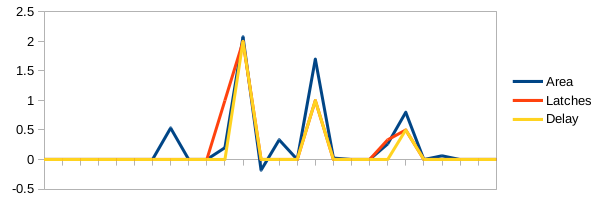
\includegraphics{graphics/diff.png}
	\caption{Difference between non- and exact solution compared by area, latches and delay.}
	\label{fig:diff}
\end{figure}

\section{Verdict}
As seen in the mapping result compared to one hot encoding binary state encoding using dichotomies delivers worse result for the target technology FPGA, when area consumption is compared. For this technology a reduction for boolean function below 5 inputs doest reduce the used area, as seen in the lut description.

\myworries{LUT description}

For example, when using a gate array target technology the amount of used logic gates and latches is reduced compared to a one hot encoding. \myworries{Reference to result table with latches}

To summaries, an exact encoding algorithm should only be used if the target technology can utilize the improved solution and when the resulting enormous runtime increase is acceptable. 

\chapter*{Results Data}

\begin{table}[h]
\centering
	\begin{tabular}{|l|r|r|r|r|}
	\hline
		\textbf{State Machine} & \textbf{Area} & \textbf{Delay} & \textbf{Latch} & \textbf{Runtime}\\
		\hline
		results\_exact/004\_dk15.kiss2.blif & 8.0 & 1.00 & 8 & 0\\
		results\_exact/004\_lion.kiss2.blif & 1.5 & 1.00 & 3 & 0\\
		results\_exact/004\_mc.kiss2.blif & 3.5 & 1.00 & 7 & 0\\
		results\_exact/004\_tav.kiss2.blif & 8.0 & 2.00 & 7 & 1\\
		results\_exact/004\_train4.kiss2.blif & 1.5 & 1.00 & 3 & 0\\
		results\_exact/005\_s8.kiss2.blif & 7.0 & 2.00 & 4 & 0\\
		results\_exact/006\_bbtas.kiss2.blif & 5.0 & 1.00 & 6 & 0\\
		results\_exact/006\_s27.kiss2.blif & 7.5 & 2.00 & 5 & 1\\
		results\_exact/007\_beecount.kiss2.blif & 10.0 & 2.00 & 8 & 0\\
		results\_exact/007\_dk14.kiss2.blif & 8.0 & 1.00 & 8 & 0\\
		results\_exact/007\_dk27.kiss2.blif & 2.5 & 1.00 & 5 & 0\\
		results\_exact/008\_dk17.kiss2.blif & 6.5 & 1.00 & 7 & 1\\
		results\_exact/008\_ex6.kiss2.blif & 30.5 & 3.00 & 12 & 0\\
		results\_exact/008\_shiftreg.kiss2.blif & 1.5 & 1.00 & 4 & 0\\
		results\_exact/009\_ex5.kiss2.blif & 5.0 & 1.00 & 6 & 1\\
		results\_exact/009\_lion9.kiss2.blif & 5.0 & 1.00 & 5 & 0\\
		results\_exact/010\_bbara.kiss2.blif & 21.0 & 3.00 & 7 & 1\\
		results\_exact/010\_ex3.kiss2.blif & 6.0 & 1.00 & 6 & 1\\
		results\_exact/010\_ex7.kiss2.blif & 5.0 & 1.00 & 6 & 0\\
		results\_exact/010\_opus.kiss2.blif & 19.0 & 3.00 & 10 & 1\\
		results\_exact/011\_train11.kiss2.blif & 10.0 & 2.00 & 6 & 13\\
		results\_exact/012\_modulo12.kiss2.blif & 2.0 & 1.00 & 5 & 1\\
		results\_exact/014\_ex4.kiss2.blif & 16.0 & 2.00 & 14 & 6\\
		results\_exact/015\_dk512.kiss2.blif & 6.5 & 1.00 & 8 & 60000\\
		results\_exact/020\_tma.kiss2.blif & 39.5 & 3.00 & 11 & 0\\
		results\_exact/024\_pma.kiss2.blif & 88.5 & 4.00 & 13 & 1\\
		\hline
	\end{tabular}
	\caption{Results of Exact Encoding Approach Using Dichotomies}
	\label{tab:exact}
\end{table}

\begin{table}[h]
\centering
	\begin{tabular}{|l|r|r|r|r|}
	\hline
		\textbf{State Machine} & \textbf{Area} & \textbf{Delay} & \textbf{Latch} & \textbf{Runtime}\\
		\hline
results\_nonexact/004\_dk15.kiss2.blif & 8.0 & 1.00 & 8 & 0 \\
results\_nonexact/004\_lion.kiss2.blif & 1.5 & 1.00 & 3 & 0 \\
results\_nonexact/004\_mc.kiss2.blif & 3.5 & 1.00 & 7 & 0 \\
results\_nonexact/004\_tav.kiss2.blif & 8.0 & 2.00 & 7 & 0 \\
results\_nonexact/004\_train4.kiss2.blif & 1.5 & 1.00 & 3 & 0 \\
results\_nonexact/005\_s8.kiss2.blif & 7.0 & 2.00 & 4 & 1 \\
results\_nonexact/006\_bbtas.kiss2.blif & 5.0 & 1.00 & 6 & 0 \\
results\_nonexact/006\_s27.kiss2.blif & 11.5 & 2.00 & 5 & 0 \\
results\_nonexact/007\_beecount.kiss2.blif & 10.0 & 2.00 & 8 & 0 \\
results\_nonexact/007\_dk14.kiss2.blif & 8.0 & 1.00 & 8 & 0 \\
results\_nonexact/007\_dk27.kiss2.blif & 3.0 & 1.00 & 6 & 0 \\
results\_nonexact/008\_dk17.kiss2.blif & 20.0 & 3.00 & 9 & 0 \\
results\_nonexact/008\_ex6.kiss2.blif & 25.0 & 3.00 & 12 & 0 \\
results\_nonexact/008\_shiftreg.kiss2.blif & 2.0 & 1.00 & 4 & 0 \\
results\_nonexact/009\_ex5.kiss2.blif & 5.0 & 1.00 & 6 & 1 \\
results\_nonexact/009\_lion9.kiss2.blif & 13.5 & 2.00 & 6 & 0 \\
results\_nonexact/010\_bbara.kiss2.blif & 21.5 & 3.00 & 7 & 0 \\
results\_nonexact/010\_ex3.kiss2.blif & 6.0 & 1.00 & 6 & 0 \\
results\_nonexact/010\_ex7.kiss2.blif & 5.0 & 1.00 & 6 & 0 \\
results\_nonexact/010\_opus.kiss2.blif & 24.0 & 3.00 & 11 & 0 \\
results\_nonexact/011\_train11.kiss2.blif & 18.0 & 3.00 & 7 & 0 \\
results\_nonexact/012\_modulo12.kiss2.blif & 2.0 & 1.00 & 5 & 0 \\
results\_nonexact/013\_s386.kiss2.blif & 42.0 & 3.00 & 12 & 0 \\
results\_nonexact/014\_ex4.kiss2.blif & 17.0 & 2.00 & 14 & 1 \\
results\_nonexact/015\_dk512.kiss2.blif & 6.5 & 1.00 & 8 & 0 \\
results\_nonexact/015\_mark1.kiss2.blif & 46.0 & 4.00 & 26 & 0 \\
results\_nonexact/016\_bbsse.kiss2.blif & 32.0 & 3.00 & 12 & 1 \\
results\_nonexact/016\_cse.kiss2.blif & 60.5 & 4.00 & 13 & 0 \\
results\_nonexact/016\_kirkman.kiss2.blif & 43.0 & 4.00 & 11 & 1 \\
results\_nonexact/016\_sse.kiss2.blif & 48.5 & 4.00 & 13 & 0 \\
results\_nonexact/018\_s208.kiss2.blif & 61.0 & 4.00 & 8 & 2 \\
results\_nonexact/018\_s420.kiss2.blif & 44.0 & 4.00 & 7 & 2 \\
results\_nonexact/019\_ex2.kiss2.blif & 19.0 & 3.00 & 7 & 1 \\
results\_nonexact/019\_keyb.kiss2.blif & 65.0 & 5.00 & 8 & 4 \\
results\_nonexact/020\_ex1.kiss2.blif & 77.5 & 4.00 & 26 & 4 \\
results\_nonexact/020\_s1a.kiss2.blif & 109.0 & 4.00 & 14 & 6 \\
results\_nonexact/020\_s1.kiss2.blif & 119.0 & 5.00 & 13 & 11 \\
results\_nonexact/020\_tma.kiss2.blif & 39.5 & 3.00 & 11 & 0 \\
results\_nonexact/024\_donfile.kiss2.blif & 19.5 & 3.00 & 6 & 66 \\
results\_nonexact/024\_pma.kiss2.blif & 88.5 & 4.00 & 13 & 0 \\
results\_nonexact/025\_s820.kiss2.blif & 153.5 & 6.00 & 27 & 393 \\
results\_nonexact/025\_s832.kiss2.blif & 158.0 & 6.00 & 28 & 452 \\
results\_nonexact/027\_dk16.kiss2.blif & 60.0 & 3.00 & 10 & 1243 \\
		\hline
	\end{tabular}
	\caption{Results of Non-Exact Encoding Approach Using Dichotomies}
\end{table}




\end{document}
